%----------------------------------------------------------------------------
\chapter{Jegyzőkönyv}
%----------------------------------------------------------------------------
%----------------------------------------------------------------------------
\section{A labor témája}
%----------------------------------------------------------------------------
A mérés során egy MIMO lepárlótorony robusztus irányítását valósítottam meg Matlab Robust Control Toolboxa és annak felhasználásával előre megírt szkriptek segítségével. Ezen szkriptek között található a mod\_col függvény, mely a desztillációs torony modelljének munkaponti linearizációjával képes a redukálni a modellt. A mérést ezen redukált modellen, a \figref{System}~ábrán látható zárt rendszeren végeztem.

\begin{figure}[!ht]\hspace{1mm}
	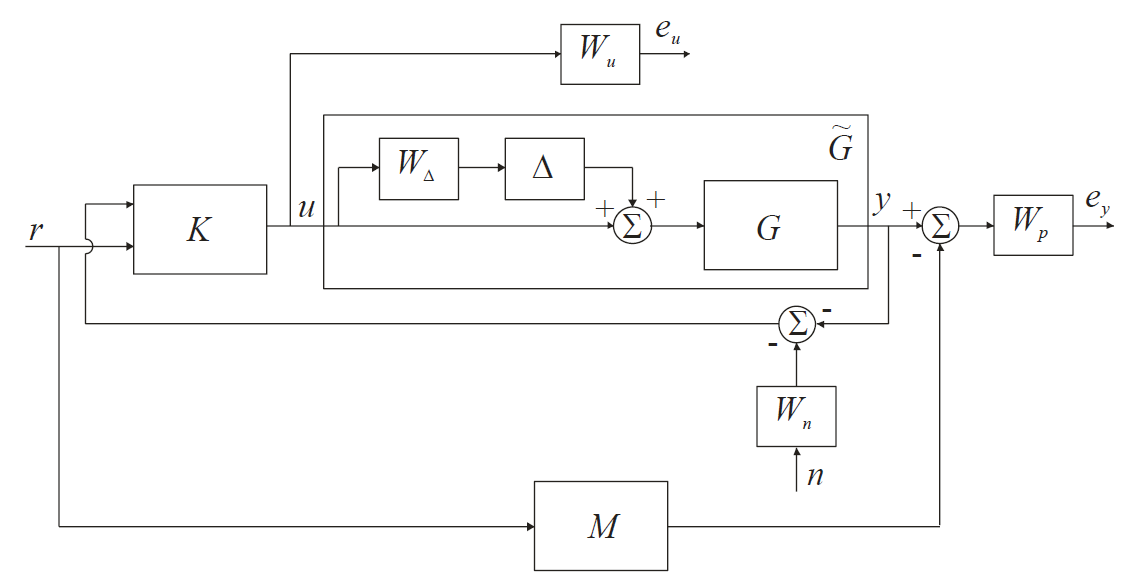
\includegraphics[width=140mm,keepaspectratio]{figures/2m06/system.png}
	\caption{A zárt kör folyamatábrája}
	\label{fig:System}
\end{figure}
\newpage
%----------------------------------------------------------------------------
\section{Első feladat}
%----------------------------------------------------------------------------
A mérésvezető által meghatározott {$k_i \in$ [0.9 1.1], $\Theta_i \in$ [0 1]} bizonytalanság és késleltetés mellett inicializáltam a linearizált modellt az \textit{olp\_col} függvénnyel. 

\begin{figure}[!ht]
	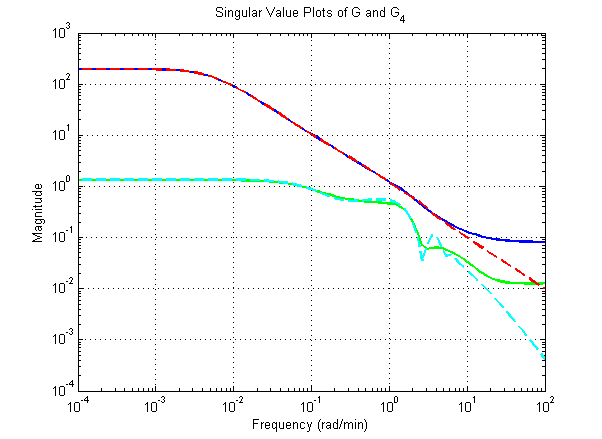
\includegraphics[width=75mm,keepaspectratio]{figures/2m06/olp_old_1_.png}
	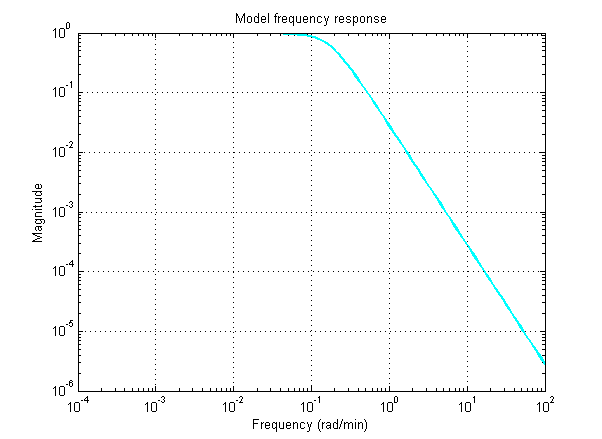
\includegraphics[width=75mm,keepaspectratio]{figures/2m06/olp_old_2_.png}
	\caption{A zárt rendszer frekvencia válasza}
	\label{fig:Init}
\end{figure}

A mérési útmutatóban található súlyozó függvény alapján a \textit{hin\_col} paranccsal megterveztem a szabályzót, mely a \figref{HinOld}~ábrán látható. Ezután leszimuláltam a megadott bizonytalanságok alapján a rendszert, melynek tranziensei a \figref{PrtOld1}~ábrán és a \figref{PrtOld2}~ábrán láthatóak, attól függően, hogy az első vagy a második bemenethez tartozó alapjelre adtunk egységugrást.

\begin{figure}[!ht]\hspace{36mm}
	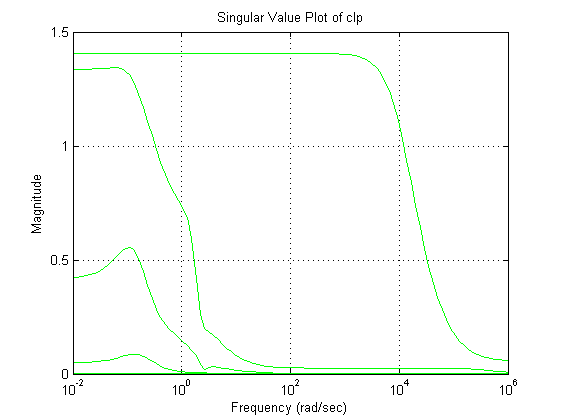
\includegraphics[width=75mm,keepaspectratio]{figures/2m06/hin_old_.png}
		\caption{A megvalósított szabályzó}
	\label{fig:HinOld}
\end{figure}
\begin{figure}[!ht]
	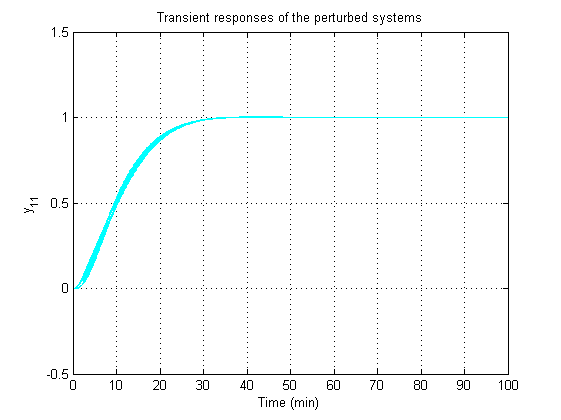
\includegraphics[width=75mm,keepaspectratio]{figures/2m06/prt_old_1.png}
	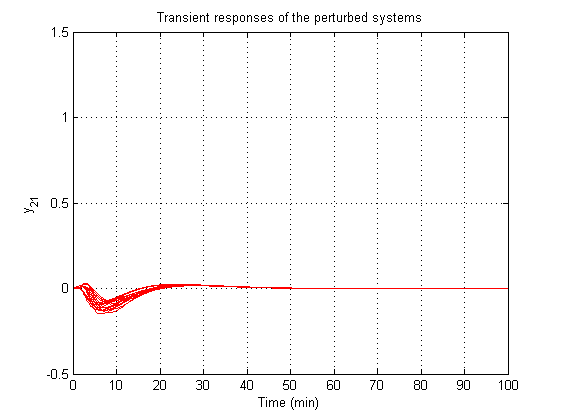
\includegraphics[width=75mm,keepaspectratio]{figures/2m06/prt_old_2.png}\vspace{2mm}
	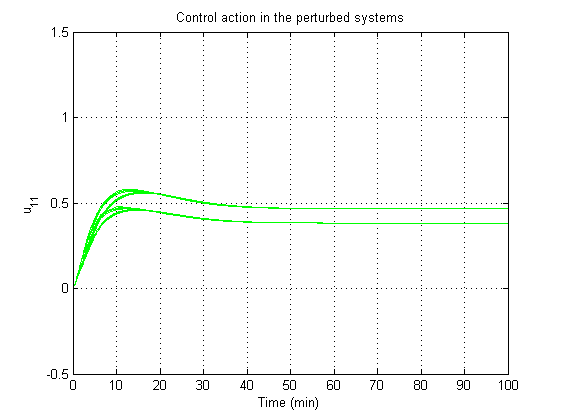
\includegraphics[width=75mm,keepaspectratio]{figures/2m06/prt_old_3.png}
	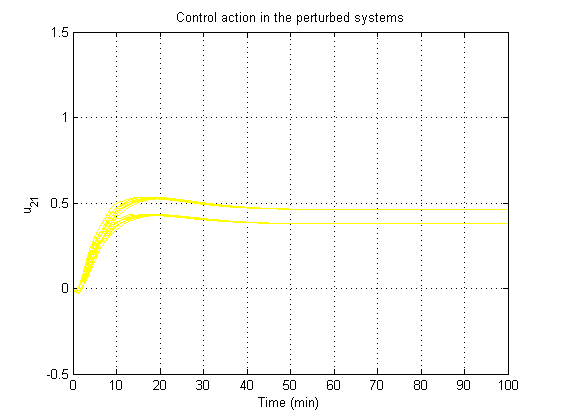
\includegraphics[width=75mm,keepaspectratio]{figures/2m06/prt_old_4.png}
		\caption{A rendszer beavatkozó jelei és kimenetei, az első alapjelhez tartozó egységugrás esetén}
	\label{fig:PrtOld1}
\end{figure}
\begin{figure}[!ht]
	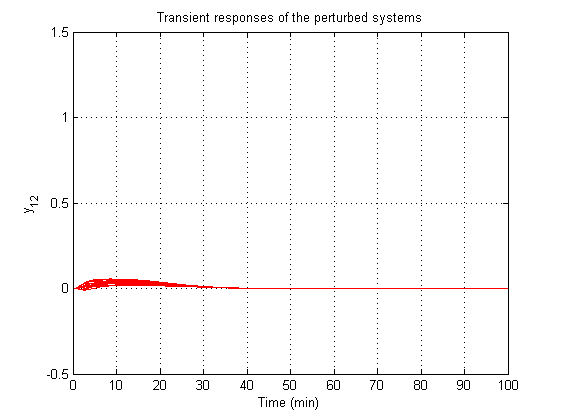
\includegraphics[width=75mm,keepaspectratio]{figures/2m06/prt_old_5.png}
	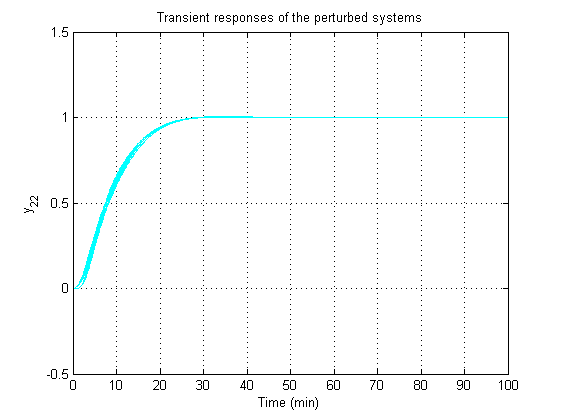
\includegraphics[width=75mm,keepaspectratio]{figures/2m06/prt_old_6.png}\vspace{2mm}
	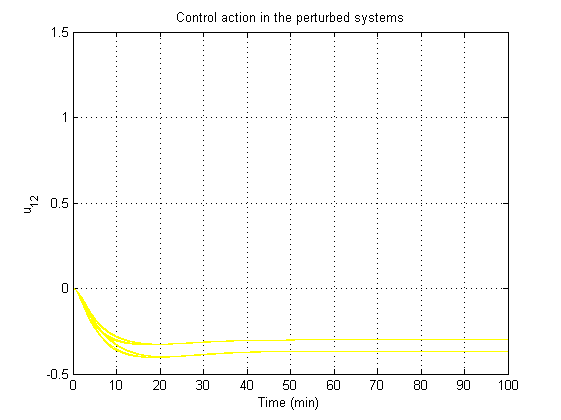
\includegraphics[width=75mm,keepaspectratio]{figures/2m06/prt_old_7.png}
	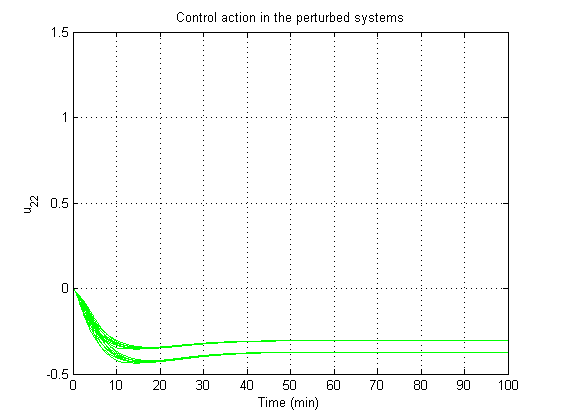
\includegraphics[width=75mm,keepaspectratio]{figures/2m06/prt_old_8.png}
		\caption{A rendszer beavatkozó jelei és kimenetei, a második alapjelhez tartozó egységugrás esetén}
	\label{fig:PrtOld2}
\end{figure}

\newpage
%----------------------------------------------------------------------------
\section{Második feladat}
%----------------------------------------------------------------------------

A rendszer bizonytalanságát növelve az első feladatban megvalósított szabályzó már nem lesz elég robusztus, és elveszti a stabilitását. Erre láthatóak példák a \figref{PrtMod}~ábrán, melyeken az elsőn egy enyhén, a másodikon egy erősen szélesebb bizonytalanságot és késleltetést állítottam be.
A beállított paraméterek értékei:
\begin{itemize}
	\item Enyhébb eset: {$k_i \in$ [0.7 1.3], $\Theta_i \in$ [0 1.07]}
	\item Erősebb eset: {$k_i \in$ [0.65 1.35], $\Theta_i \in$ [0 1.1]}
\end{itemize}

\begin{figure}[!ht]
	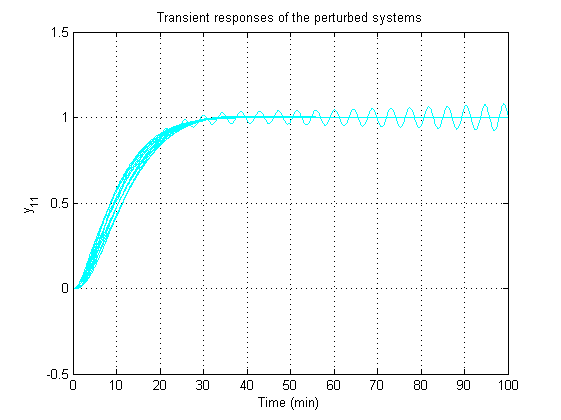
\includegraphics[width=75mm,keepaspectratio]{figures/2m06/prt_small_1.png}
	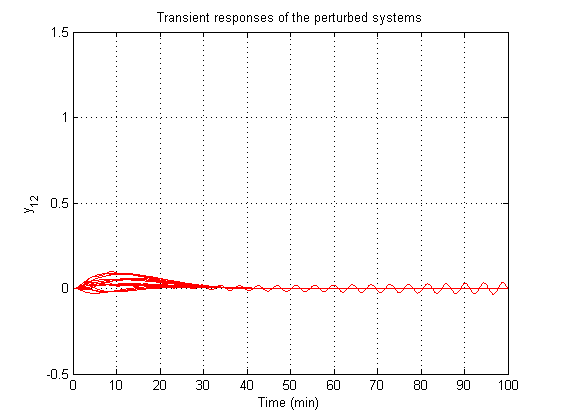
\includegraphics[width=75mm,keepaspectratio]{figures/2m06/prt_small_2.png}\vspace{2mm}
	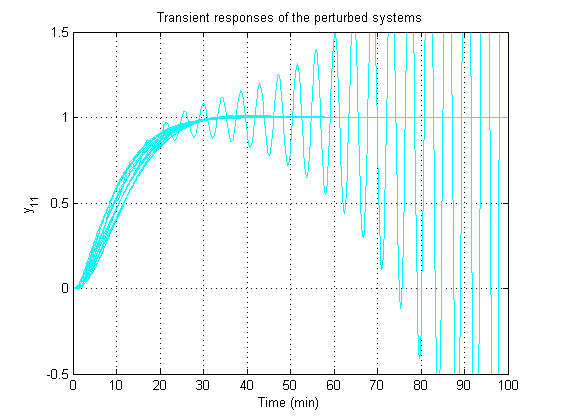
\includegraphics[width=75mm,keepaspectratio]{figures/2m06/prt_big_1.png}
	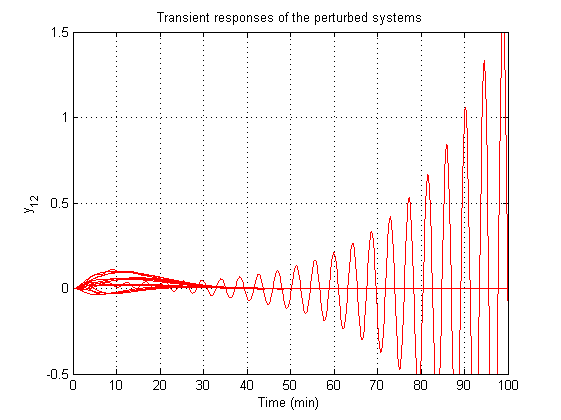
\includegraphics[width=75mm,keepaspectratio]{figures/2m06/prt_big_2.png}
		\caption{A rendszer válaszának tranziensei szélesebb bizonytalanságot feltételezve}
	\label{fig:PrtMod}
\end{figure}

\newpage
%----------------------------------------------------------------------------
\section{Harmadik feladat}
%----------------------------------------------------------------------------
Az új szabályzót az előző feladatban bemutatott, enyhén növelt bizonytalansági feltételek mellett terveztem meg. Ehhez az \textit{unc\_col} függvényt hívtam meg, melyben előzetesen módosítottam a késleltetést és a bizonytalanságot, így az már az új feltételekből kapott görbeseregeket jeleníti meg. A \textit{wfit} parancs segítségével ezekhez új súlyozó függvényt tudtam keresni, mely a következő lett:
\begin{equation}\label{NewWeight}
\frac{2.3509    s^{3}+8.4222   s^{2}+13.6532s+    3.0960}{s^{3}+4.6982  s^{2}+ 10.2369    s+9.4826}
\end{equation}

A \textit{wts\_col} fájlt ezek alapján fel is frissítettem, majd újraszimuláltam a rendszert.


Amint azt a \figref{PrtNew}~ábrán is látni, az új szabályzó a kibővített bizonytalansági feltételek mellett képes volt javítani a rendszer ugrásválaszán, ám nem minden oszcillációt sikerült megszüntetni. Ezen az eredményen további súlyozó függvények kipróbálása mellett a $W_n$ és $W_p$ mátrixok módosításával lehet javítani.



\begin{figure}[!ht]
	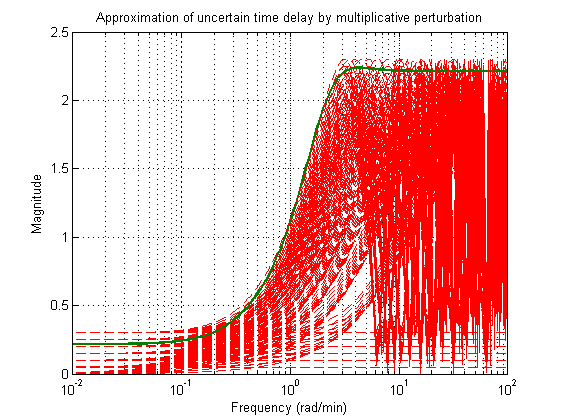
\includegraphics[width=75mm,keepaspectratio]{figures/2m06/unc_col_before.png}
	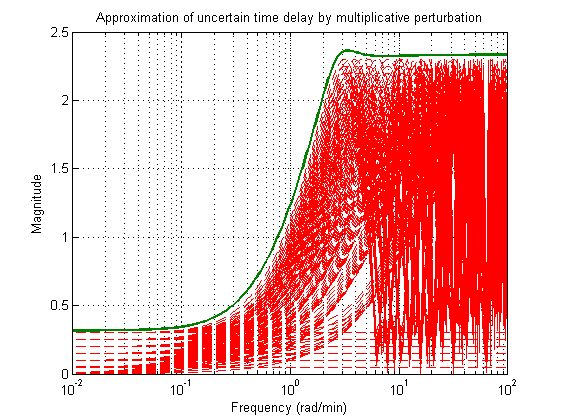
\includegraphics[width=75mm,keepaspectratio]{figures/2m06/unc_col_after.png}
	\caption{Új súlyozó függvény felvétele}
	\label{fig:Unc}
\end{figure}



\begin{figure}[!ht]
	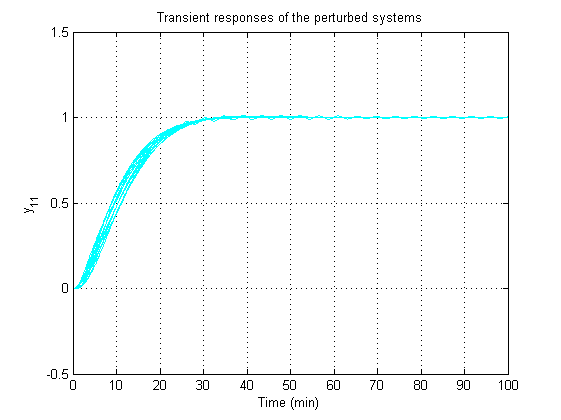
\includegraphics[width=75mm,keepaspectratio]{figures/2m06/prt_new_1_.png}
	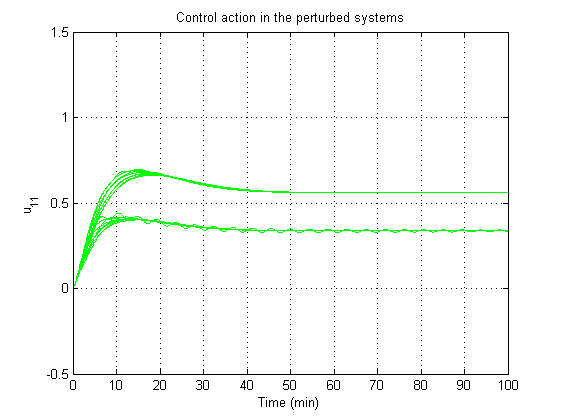
\includegraphics[width=75mm,keepaspectratio]{figures/2m06/prt_new_3_.png}
	\caption{Az új szabályzó viselkedése a kibővített bizonytalansági feltételek mellett}
	\label{fig:PrtNew}
\end{figure}




